\documentclass[12pt, a4paper,oneside]{book}
\newcommand{\re}{\mathrm{e}}
\newcommand{\ri}{\mathrm{i}}
\newcommand{\rd}{\mathrm{d}}
\def\semicolon{\nobreak\mskip2mu\mathpunct{}\nonscript\mkern-\thinmuskip{;}
\mskip6muplus1mu\relax} % This defines the semicolon command

        % allows index generation
\usepackage{graphicx}        % standard LaTeX graphics tool
                             % when including figure files
\usepackage{multicol}        % used for the two-column index

\usepackage{color,tikz}

\usepackage{amsmath,eucal,amssymb}
\usepackage{mathrsfs,graphicx,texdraw}
\usepackage{fancyhdr,framed}
\usepackage{tikz, tikz-3dplot}
\usepackage{tkz-euclide}
\usetikzlibrary{decorations.fractals}
\usetikzlibrary{decorations.footprints}

\usepackage{palatino}

\usepackage[latin1]{inputenc}

\usepackage[T1]{fontenc}
%\usepackage[dvips]{graphicx}
%\usepackage{times}

\definecolor{mygreen}{HTML}{622567} %%% Purple
\definecolor{Gray}{HTML}{333333} %%% Gray

\definecolor{myred}{HTML}{D55C19} %%%EssexOrange
\definecolor{myblue}{HTML}{007A87} %%%Seagrass
\definecolor{Mint}{HTML}{35C4B5} %%% Mint

\def\grole{\mathrel{\mathchoice {\vcenter{\offinterlineskip\halign{\hfil
$\displaystyle##$\hfil\cr>\cr\noalign{\vskip-1.5pt}<\cr}}}
{\vcenter{\offinterlineskip\halign{\hfil$\textstyle##$\hfil\cr
>\cr\noalign{\vskip-1.5pt}<\cr}}}
{\vcenter{\offinterlineskip\halign{\hfil$\scriptstyle##$\hfil\cr
>\cr\noalign{\vskip-1pt}<\cr}}}
{\vcenter{\offinterlineskip\halign{\hfil$\scriptscriptstyle##$\hfil\cr
>\cr\noalign{\vskip-0.5pt}<\cr}}}}}

\newenvironment{rcases}
  {\left.\begin{aligned}}
  {\end{aligned}\right\rbrace}

\newenvironment{lcases}
  {\left\lbrace\begin{aligned}}
  {\end{aligned}\right.}

\newtheorem{theorem}{Theorem}[section]
\newtheorem{lemma}[theorem]{Lemma}
\newtheorem{proposition}[theorem]{Proposition}
\newtheorem{corollary}[theorem]{Corollary}
\newtheorem{definition}[theorem]{Definition}
\newtheorem{example}[theorem]{Example}
\newtheorem{remark}[theorem]{Remark}

\newenvironment{proof}[1][Proof]{\begin{trivlist}
\item[\hskip \labelsep {\bfseries #1}]}{\end{trivlist}}
\newenvironment{solution}[1][Solution]{\begin{trivlist}
\item[\hskip \labelsep {\bfseries #1}]}{\end{trivlist}}

\newcommand{\qed}{\nobreak \ifvmode \relax \else
      \ifdim\lastskip<1.5em \hskip-\lastskip
      \hskip1.5em plus0em minus0.5em \fi \nobreak
      \vrule height0.75em width0.5em depth0.25em\fi}

\numberwithin{equation}{section}
\def\Ad{{\mbox{Ad}}}
\def\im{{\mbox{Im}}}
\def\Re{{\mbox{Re}\;}}
\def\ad{\mathrm{ad\,}}
\def\openone{\leavevmode\hbox{\small1\kern-3.3pt\normalsize1}}
\def\Res{\mathop{\mbox{Res}\,}\limits}
\def\biglb{\big[\hspace*{-.7mm}\big[}
\def\bigrb{\big]\hspace*{-.7mm}\big]}

\def\bigrbt{\mathop{\bigrb }\limits_{\widetilde{\;}}}
\def\biggrbt{\mathop{\biggrb }\limits_{\widetilde{\;}}}
\def\Bigrbt{\mathop{\Bigrb }\limits_{\widetilde{\;}}}
\def\Biggrbt{\mathop{\Biggrb }\limits_{\widetilde{\;}}}

\def\bPhi{\mathbf{\Phi}}
\def\bM{\mathbf{M}}
\def\bm{\mathbf{m}}
\def\bbbc{{\Bbb C}}
\def\bbbr{{\Bbb R}}
\def\bbbz{{\Bbb Z}}
\def\bbbs{{\Bbb S}}
\def\diag{\mbox{diag}\,}
\def\tr{\mbox{tr}\,}

\textwidth=17cm   \textheight=24.5cm \voffset=-2cm

\evensidemargin=-0.5cm \oddsidemargin=-0.5cm

 \renewcommand{\baselinestretch}{1.5}

%%%%%%%%fancy header%%%%%%%%%%%%%%%%%

\usepackage{fancyhdr}
\pagestyle{fancy}
\usepackage{calc}
\newlength{\pageoffset}
\setlength{\pageoffset}{0cm}% use whatever you like
\fancyheadoffset[LE,RO]{\pageoffset}
\renewcommand{\chaptermark}[1]{\markboth{#1}{}}
\renewcommand{\sectionmark}[1]{\markright{\thesection\ #1}}
\fancyhf{}
\fancyhead[LE]{\makebox[\pageoffset][l]{\thepage}\hfill\leftmark}
\fancyhead[RO]{\rightmark\hfill\makebox[\pageoffset][r]{\thepage}}
\fancypagestyle{plain}{%
    \fancyhead{} % get rid of headers
    \renewcommand{\headrulewidth}{0pt} % and the line
}

%%%%%%%%%%%%%%%%%%%%%%%%%%%%%%%%%%%%

\arraycolsep=2pt

%%%%Fancy Chapter%%%

%\usepackage{lmodern}
\usepackage{graphicx}
\usepackage{xcolor}
\usepackage{titlesec}
\usepackage{microtype}
\usepackage{lipsum}

%\definecolor{myblue}{RGB}{0,82,155}

\titleformat{\chapter}[display]
  {\normalfont\bfseries\color{myred}}
  {\filleft\hspace*{-60pt}%
    \rotatebox[origin=c]{90}{%
      \normalfont\color{black}\Large%
        \textls[180]{\textsc{\chaptertitlename}}%
    }\hspace{10pt}%
    {\setlength\fboxsep{0pt}%
    \colorbox{myred}{\parbox[c][3cm][c]{2.5cm}{%
      \centering\color{white}\fontsize{80}{90}\selectfont\thechapter}%
    }}%
  }
  {10pt}
  {\titlerule[2.5pt]\vskip3pt\titlerule\vskip4pt\LARGE\sffamily}

% hyperref should be loaded after all other packages
% aliascnt is needed to get \autoref (from hyperref) to work correctly with custom amsthm theorems
\usepackage{aliascnt}
\usepackage[colorlinks,linkcolor=myblue,citecolor=mygreen]{hyperref}

\begin{document}

\thispagestyle{empty}

\begin{minipage}{0.2\textwidth}
\centerline{\includegraphics[width=.4\textwidth]{essex} }
\end{minipage}
\begin{minipage}{0.8\textwidth}

$ \qquad \qquad \qquad ${\LARGE \bf \sl University of Essex}

{\LARGE \bf Department of Mathematical Sciences}

\end{minipage}

\begin{center}

\noindent\textcolor{myred}{\rule{\linewidth}{4.8pt}}

\vspace{1cm}

{\LARGE \sc  MA838: Capstone  Project Dissertation}

\vspace{1.5cm}

{\Huge{\color{myblue}  Communicating Mathematics \\ and Data Science}}

\vspace{1.5cm}

{\Large \bf Karen Yim \\ 1705960}

\vspace{1.5cm}

\centerline{\includegraphics[width=1\textwidth]{Figure}}

\vspace{1.5cm}

{\Large {Supervisor:} {\color{mygreen} \bf Dr. Joe Bailey}}

\vspace{.25cm}

\noindent\textcolor{myred}{\rule{\linewidth}{4.8pt}}

\vspace{1cm}
{\Large \ March 2022 }\\[4pt]
{\Large Colchester}
\end{center}
\newpage
\tableofcontents

\listoffigures
\listoftables

\chapter{Acknowledgements}
I would like to thank my supervisor Dr. Joe Bailey for his guidance and support during the period of writing my dissertation, my personal tutors Dr. Jess Claridge and Professor Peter Higgins for supporting me throughout the course of the degree and their advice to help me get to where I am today and finishing my modules and this project in time.

\chapter{Project Overview}\label{ch:x}


\chapter{Abstract}\label{ch:x}
Abstract (500 words roughly), brief rationale (meaning behind) why are you doing the study, method (explain audience, age, whatever, like experiment), results (data findings), discussions (conclusions, explain what the findings mean in context, how is it applied to the research project), limitations (what would you do to improve, or further research)

\chapter{Introduction}\label{ch:x}

You can start with some introduction of your project and background.


You can make figures  from files as you can see in Figure \ref{fig:A3.1}. For this you need to use include graphics.

\begin{figure}[htb]
\centerline{\includegraphics[width=1\textwidth]{Figure}}
\caption{The Gauss map $\mathbf{g}_{K}$ takes $x\in \partial K$ to the outer normal $n_x\in\mathbb{S}^{n-1}$ at that point}
\label{fig:A3.1}
\end{figure}


While writing be clear and precise and give references whenever necessary. You may like to use theorem, definition, lemma, and example environments provided by \LaTeX. For example,

Pioneering work of Emmy Noether \cite{Noether} provides a connection between symmetries and conservation laws. This result, known as Noether's theorem states that

\begin{theorem}[Noether, \cite{Noether}]
Every differentiable symmetry of the action of a physical system has a corresponding conservation law.
\end{theorem}

\begin{example}
This is an example.
\end{example}

\begin{lemma}
This is a lemma.
\end{lemma}

\begin{definition}
In 1950, Alan Turing published an article \cite{Turing} in \textit{Mind}
titled ``Computing Machinery and Intelligence'' where he considered the question ``Can machines think?''. This is known as {\bf Turing's Test}.
\end{definition}

\begin{remark}
This is a very important remark.
\end{remark}

You can also make figures  using \LaTeX packages for figures (e.g. the {\tt TikZ package}) as you can see in Figure \ref{fig:tikz}.

\begin{figure}[htb]
\begin{center}
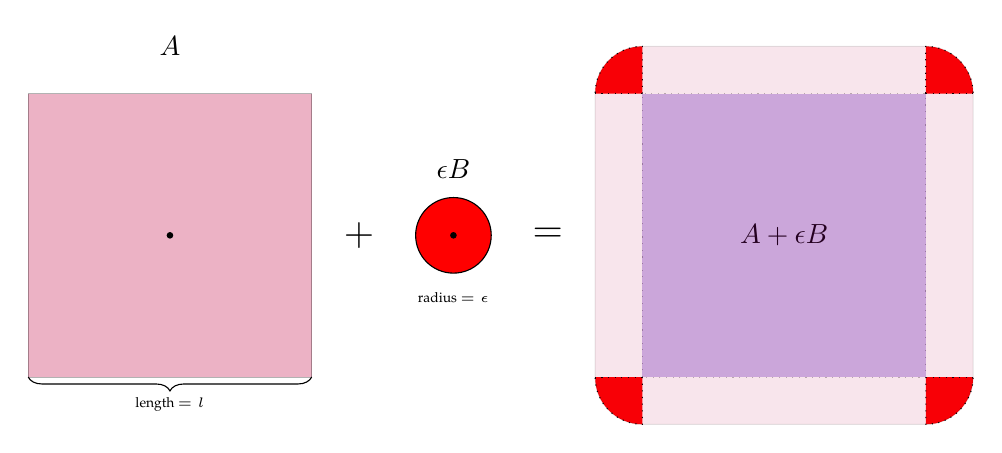
\begin{tikzpicture}[scale=.6]
\draw[fill=purple, opacity=.3] (-3,-3) rectangle (3,3);
\fill (0,0) circle [radius=2pt];
\node at (0,4) {$A$};
\node at (4,0) {\Large $+$};
\draw[fill=red] (6,0) circle (.8cm);
\fill (6,0) circle [radius=2pt];
\node[above] at (6,1) {$\epsilon B$};
\node[below] at (6,-1) {\tiny radius $=\epsilon$};
\node at (8,0) {\Large $=$};

\draw [decorate,decoration={brace,amplitude=5pt, mirror}]
(-3,-3) -- (3,-3) node[below] [black,midway, yshift=-4pt] {\tiny length $=l$};

\draw[dotted, fill=blue, opacity=.1] (10,-3) rectangle (16,3);

\node at (13,0) {$A +  \epsilon B$};


\draw[dotted, fill=blue, opacity=.1] (10,-3) rectangle (16,3);

\draw[dotted, fill=red] (10,-3)--(10,-4) arc (270:180:1);
\draw[dotted, fill=red] (10,3)--(10,4) arc (90:180:1);
\draw[dotted, fill=red] (16,3)--(16,4) arc (90:0:1);
\draw[dotted, fill=red] (16,-3)--(16,-4) arc (270:360:1);

\draw[dotted] (10,-3)--(9,-3);
\draw[dotted] (16,-3)--(17,-3);

\draw[dotted] (16,3)--(16,4);
\draw[dotted] (16,3)--(17,3);

\draw[dotted] (10,3)--(9,3);


\draw[dotted, fill=purple, opacity=.1] (10,-3) rectangle (16,3);
\draw[fill=purple, opacity=.1] (16,4)--(10,4) arc (90:180:1)--(9,-3)--(9,-3) arc (180:270:1)--(10,-4)--(16,-4)--(16,-4) arc (270:360:1)--(17,-3)--(17,3) arc (0:90:1);
\end{tikzpicture}
\end{center}
\caption{Minkowski sum of a square and ball with radius $\epsilon$}
\label{fig:tikz}
\end{figure}


\chapter{The national curriculum}\label{ch:x}

\section{Overview}\label{sec:x.x}

As this project is on the communication of mathematics and data science, the first and foremost important chapter is the national curriculum. As defined [1], The project aim is to create outreach activities that are suitable in engaging with students of appropriate age groups whilst adhering to the standards children should reach in mathematics. However, please note that there is not a fixed chronological order in which it must be taught at schools. As a result, teachers need to be aware that certain topics may not have been covered yet.

\section{Key Stage 3 (KS3)}\label{sec:x.x}

Key Stage 3 is the age group of 11 - 14 year olds in Year 7 - 9. My presentation for mathematics is designed in mind to be presented to Year 9 which are 13-14 year olds.

https://www.gov.uk/government/publications/national-curriculum-in-england-mathematics-programmes-of-study/national-curriculum-in-england-mathematics-programmes-of-study#key-stage-3

\section{Key Stage 4 (KS4)}\label{sec:x.x}

KS4 is where some children may take GCSEs at the age of 14-15 in Year 10, whereas majority take GCSEs or other national assessments in Year 11 at the age of 15-16.

\section{Key Stage 5 (KS5)}\label{sec:x.x}



https://assets.publishing.service.gov.uk/government/uploads/system/uploads/attachment_data/file/516949/GCE_AS_and_A_level_subject_content_for_mathematics_with_appendices.pdf


\chapter{Literature Review}\label{ch:x}

\section{Researching Pedagogy}\label{sec:x.x}

The text goes here ...

\section{Good teaching practice}\label{sec:x.x}

\section{Different teaching methods}\label{sec:x.x}

\section{Presentation}\label{sec:x.x}

\section{Pedagogy - profession of teaching}\label{sec:x.x}


\chapter{Communicating Mathematics}\label{ch:x.x}

... goes here.

\section{Preparation of communication}\label{sec:x.x}

Presentation research

\section{Making a presentation}\label{sec:x.x}

Making the presentation slides

\section{Realisation of other things to prepare}\label{sec:x.x}

Preparing a detailed handover, lesson plans, handout sheets, presentation slides

\section{Practice communication}\label{sec:x.x}

Practicing the presentation beforehand

Leading up to the the presentation that was to be presented to the origami society, I had been practicing beforehand with a friend. During this process, I was consistently making changes whilst understanding what needs to be solidified before the presentation at the origami society. I was moving a lot to practice speaking. It was more overwhelming than I had thought as I wanted to try to make it perfect. My energy was seen but my knowledge content was still lacking. Furthermore, I was rambling during the start of the introduction which meant I was taking a lot longer for the slides that were not important. In this case, I was waffling and unable to demonstrate as well as I intended to. My face was making a lot of emotions but it was not always ideal for a school situations.

\section{Reflections}\label{sec:x.x}

\chapter{Communicating Data Science}\label{ch:x}

The text goes here ...

\section{Form of communication}\label{sec:x.x}

Communicating mathematics to sixth form students in the form of a blog post.

\section{Understand how to present a blog post}\label{sec:x.x}

... goes here.

\section{Preparation of a blog post}\label{sec:x.x}


\section{Making the blog post}\label{sec:x.x}


\section{Reflections}\label{sec:x.x}

\chapter{Project Findings}\label{ch:x}


\chapter{Conclusions}\label{ch:concl}
And here is the final chapter showing how clever you are ....



% Comment the following THREE lines if you do NOT have an Appendix
\appendix
\chapter{Appendix}

\section{Detailed Handover}\label{secx.x}

Insert detailed table of lesson plan next to presentation slides

\section{Lesson Plan}\label{secx.x}

Insert lesson plan

\section{Handout sheets}\label{secx.x}

Insert handouts

\section{Presentation}\label{secx.x}

Insert presentation slides


\section{Presentation video}\label{secx.x}

Insert video link of presentation


% If you need more than one appendix, then just use another \chapter command
%\chapter{Yet Another Appendix}

\chapter{Another Appendix}

Text goes here
https://www.gov.uk/national-curriculum



\begin{thebibliography}{999}

%%% Bibliography items should be below this here %%%

\bibitem{}
Gov
\newblock The national curriculum.
\newblock{\em https://www.gov.uk/national-curriculum }

\bibitem{Noether}
E.~Noether.
\newblock Invariante {V}ariationsprobleme.
\newblock {\em Nachr. d. K{\"o}nig. Gesellsch. d. Wiss. zu G{\"o}ttingen,
  Math-phys. Klasse, {Seite 235-157}}, 1918.

\bibitem{Turing}
A.~M. Turing.
\newblock Computing machinery and intelligence.
\newblock {\em Mind}, 59:433--460, 1950.


\end{thebibliography}






\end{document}
